\section{Método, malhas e custo computacional}\label{sec:metodo}

\subsection{O transiente}
\begin{itemize}
  \item \textbf{Material:} \texttt{TPZMatUnsaturatedUPwPa} (formulação $\mathbf u$--$p_w$--$p_a$ de
    \path{docs/nao_saturado}), deformação plana, $\mathbf u$ quadrático e $p_w$, $p_a$ lineares (Taylor--Hood). Na
    variante (iii) o acoplamento hidromecânico e a fase de ar estão desligados nas equações de massa (esqueleto rígido,
    $p_a = 0$): só a equação da água evolui. Armazenamento concentrado nos vértices; $K_w = 2{,}2$~GPa.
  \item \textbf{Tempo:} Euler implícito com passo fixo de 0,1~h (bissecção do passo só se o Newton falhar, o que não
    ocorreu), Newton com o jacobiano consistente, solver direto (LU esparsa).
  \item \textbf{Superfície:} fluxo $I_r$ por metro inclinado com a condição unilateral $p_w \le 0$: o nó em que $p_w$
    chegaria a 0 passa a face de percolação ($p_w = 0$) e volta ao fluxo quando a vazão pedida fica abaixo de $I_r$.
  \item \textbf{Malha} (Fig.~\ref{fig:malhas}): \texttt{tri2}, a malha estruturada de triângulos retângulos com catetos
    de 10~m dividida duas vezes: catetos de 2,5~m, \nTriTrans{} triângulos, 319 nós, 3032 equações (com $\mathbf u$,
    $p_w$ e $p_a$; a mesma nas três variantes).
\end{itemize}

\subsection{O fator de segurança: SRM}
\begin{itemize}
  \item \textbf{Definição:} o FS é o fator $F$ que leva o talude ao colapso quando a resistência é reduzida para
    $c'/F$ e $\tan\varphi'/F$ (redução de resistência, SRM). Com $\chi = 1$, a parcela da sucção, $\chi\,s\tan\varphi'$,
    cai junto: é o $\tan\varphi^b/F$ do Bishop, o mesmo fator do equilíbrio limite do artigo.
  \item \textbf{Pressões congeladas:} em cada instante, $p_w$ (e $p_a$ na variante i) do transiente é interpolada
    linearmente da malha do transiente para os nós da malha do fator e fica fixa; o fator resolve só o equilíbrio.
  \item \textbf{Material do fator:} Mohr--Coulomb associado ($\psi = \varphi'$), retorno analítico e tangente
    consistente (\texttt{TPZPlasticStepVoigt<TPZYCMohrCoulombPV2>}), $E = 20$~MPa, $\nu = 0{,}3$; $\mathbf u$
    quadrático. Cada análise parte do estado sem tensões.
  \item \textbf{Caminho:} (1) o peso é aplicado de 0 a 1 com $F = F_0 = 0{,}8$ (se o talude não ficar em pé, $F_0/2$ e
    $F_0/4$); (2) $F$ cresce por \emph{arc-length} cilíndrico (Box~4.4 de de Souza Neto et al.\ 2008), com a carga
    tangente $-\partial R/\partial F$ por diferença finita. O caminho termina num patamar (um passo aceito que sobe
    $F$ menos que 0,001, medido com o arco pedido) ou em 100 passos. O FS é o maior $F$ do caminho. Sem pontos
    plásticos a carga tangente é nula: passos de Newton com $F$ 10\,\% maior (metade quando não converge).
  \item \textbf{Refinamento adaptativo, refeito do zero em cada instante:} malha grossa \texttt{tri1} (catetos de
    5~m, \nTriFatorZero{} triângulos depois do refinamento do instante 0) e 4 níveis. Em cada nível, os elementos com
    $\sqrt{J_2(\boldsymbol\varepsilon^p)} \ge 0{,}1$ do maior (a banda de cisalhamento) são divididos (o lado cai à
    metade, com o fechamento da conformidade), e o SRM é refeito na malha nova. O FS é o do último nível; o menor
    cateto chega a 0,31~m (Fig.~\ref{fig:malhas}). A Tabela~\ref{tab:niveis} mostra o FS de cada nível em 24~h.
\end{itemize}

\begin{figure}[H]\centering
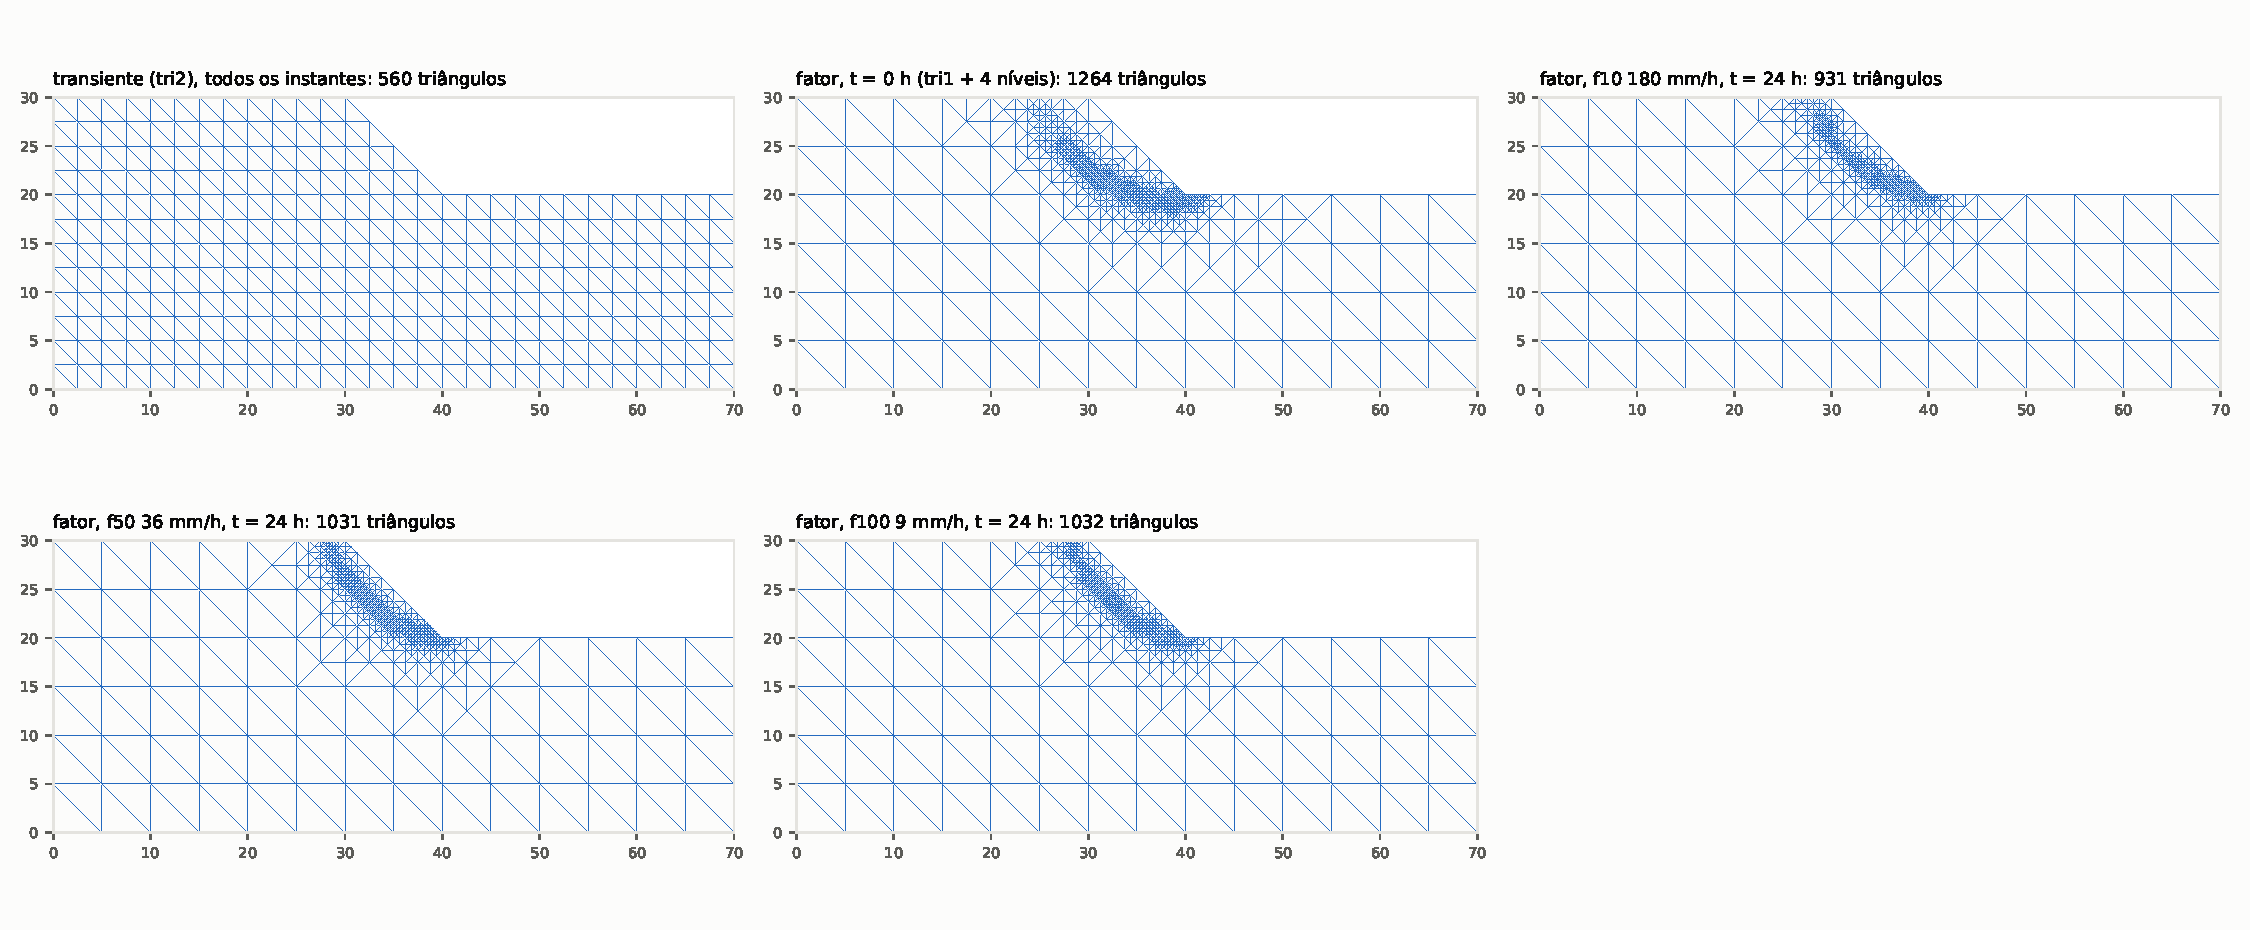
\includegraphics[width=\textwidth]{figs/malhas.pdf}
\caption{As malhas: a do transiente (a mesma em todos os instantes e casos) e a do fator no instante inicial e em
24~h em três casos: o refinamento acompanha a banda de ruptura de cada instante.}\label{fig:malhas}
\end{figure}

\begin{table}[H]\centering\small
\caption{Convergência do FS com o refinamento adaptativo do fator, em $t = 24$~h: o FS na malha grossa (tri1) e
depois de cada nível; a última coluna é a mudança do último nível.}\label{tab:niveis}
\begin{tabular}{llc ccccc c}
\toprule
solo & $I_r$ & var. & tri1 & +1 & +2 & +3 & +4 & (+3) $-$ (+4)\\
\midrule
f10 & 36 & (iii) & 1{,}660 & 1{,}548 & 1{,}506 & 1{,}491 & 1{,}485 & 0{,}006\\
f10 & 36 & (ii) & 1{,}666 & 1{,}554 & 1{,}511 & 1{,}495 & 1{,}489 & 0{,}006\\
f10 & 36 & (i) & 1{,}660 & 1{,}548 & 1{,}506 & 1{,}490 & 1{,}483 & 0{,}007\\
f10 & 90 & (iii) & 1{,}251 & 1{,}131 & 1{,}089 & 1{,}076 & 1{,}071 & 0{,}004\\
f10 & 90 & (ii) & 1{,}255 & 1{,}137 & 1{,}095 & 1{,}081 & 1{,}077 & 0{,}004\\
f10 & 90 & (i) & 1{,}254 & 1{,}142 & 1{,}099 & 1{,}084 & 1{,}078 & 0{,}006\\
f10 & 180 & (iii) & 1{,}013 & 0{,}920 & 0{,}871 & 0{,}851 & 0{,}842 & 0{,}009\\
f10 & 180 & (ii) & 1{,}013 & 0{,}920 & 0{,}871 & 0{,}852 & 0{,}843 & 0{,}009\\
f10 & 180 & (i) & 1{,}069 & 0{,}975 & 0{,}926 & 0{,}906 & 0{,}896 & 0{,}009\\
\midrule
f50 & 9 & (iii) & 1{,}934 & 1{,}829 & 1{,}803 & 1{,}789 & 1{,}786 & 0{,}003\\
f50 & 9 & (ii) & 1{,}943 & 1{,}836 & 1{,}811 & 1{,}797 & 1{,}793 & 0{,}004\\
f50 & 9 & (i) & 1{,}806 & 1{,}701 & 1{,}677 & 1{,}666 & 1{,}662 & 0{,}004\\
f50 & 36 & (iii) & 1{,}229 & 1{,}119 & 1{,}064 & 1{,}044 & 1{,}034 & 0{,}010\\
f50 & 36 & (ii) & 1{,}249 & 1{,}150 & 1{,}096 & 1{,}074 & 1{,}065 & 0{,}009\\
f50 & 36 & (i) & 1{,}095 & 1{,}000 & 0{,}951 & 0{,}928 & 0{,}919 & 0{,}009\\
f50 & 90 & (iii) & 0{,}999 & 0{,}910 & 0{,}864 & 0{,}842 & 0{,}832 & 0{,}009\\
f50 & 90 & (ii) & 1{,}077 & 0{,}991 & 0{,}940 & 0{,}917 & 0{,}906 & 0{,}011\\
f50 & 90 & (i) & 1{,}084 & 0{,}990 & 0{,}941 & 0{,}920 & 0{,}910 & 0{,}009\\
\midrule
f100 & 3{,}6 & (iii) & 2{,}016 & 1{,}927 & 1{,}907 & 1{,}894 & 1{,}889 & 0{,}005\\
f100 & 3{,}6 & (ii) & 2{,}023 & 1{,}933 & 1{,}913 & 1{,}901 & 1{,}896 & 0{,}005\\
f100 & 3{,}6 & (i) & 1{,}888 & 1{,}795 & 1{,}767 & 1{,}758 & 1{,}754 & 0{,}004\\
f100 & 9 & (iii) & 1{,}702 & 1{,}653 & 1{,}597 & 1{,}571 & 1{,}560 & 0{,}011\\
f100 & 9 & (ii) & 1{,}714 & 1{,}663 & 1{,}612 & 1{,}587 & 1{,}574 & 0{,}013\\
f100 & 9 & (i) & 1{,}474 & 1{,}380 & 1{,}317 & 1{,}292 & 1{,}279 & 0{,}013\\
f100 & 36 & (iii) & 1{,}612 & 1{,}543 & 1{,}483 & 1{,}456 & 1{,}444 & 0{,}012\\
f100 & 36 & (ii) & 1{,}622 & 1{,}552 & 1{,}492 & 1{,}466 & 1{,}452 & 0{,}014\\
f100 & 36 & (i) & 1{,}391 & 1{,}293 & 1{,}234 & 1{,}209 & 1{,}198 & 0{,}010\\
\bottomrule
\end{tabular}

\end{table}

\begin{table}[H]\centering\scriptsize\setlength{\tabcolsep}{3.5pt}
\caption{Custo computacional por caso: equações, passos, iterações de Newton (total e por passo) e tempo do
transiente; faixa de equações e tempo por FS nas 49 análises do fator (média e mínimo--máximo); tempo total. PC com
Intel i7-10700K (8 núcleos, 16 threads), com 18 processos seriais ao mesmo tempo (os tempos estão inflados pela
disputa: rodando sozinho, um FS leva $\approx 12$~s).}\label{tab:custo}
\begin{tabular}{llc ccccc ccc c}
\toprule
 & & & \multicolumn{5}{c}{transiente} & \multicolumn{3}{c}{fator (49 instantes)} & \\
\cmidrule(lr){4-8}\cmidrule(lr){9-11}
solo & $I_r$ & var. & equações & passos & Newton & Newton/passo & s & equações & s/FS & s/FS (mín--máx) & s total\\
\midrule
f10 & 36 & (iii) & 3032 & 480 & 2007 & 4{,}2 & 116 & 4926--7174 & 53 & 41--98 & 2727\\
f10 & 90 & (iii) & 3032 & 480 & 2232 & 4{,}7 & 124 & 4414--6740 & 41 & 28--65 & 2150\\
f10 & 180 & (iii) & 3032 & 480 & 2400 & 5{,}0 & 131 & 4544--6504 & 36 & 21--65 & 1918\\
\midrule
f50 & 9 & (iii) & 3032 & 480 & 1937 & 4{,}0 & 114 & 5546--7172 & 56 & 43--85 & 2890\\
f50 & 36 & (iii) & 3032 & 480 & 2184 & 4{,}5 & 122 & 4302--6504 & 38 & 29--64 & 1999\\
f50 & 90 & (iii) & 3032 & 480 & 2230 & 4{,}6 & 125 & 3992--6504 & 33 & 22--66 & 1771\\
\midrule
f100 & 3{,}6 & (iii) & 3032 & 480 & 1925 & 4{,}0 & 114 & 5466--6974 & 58 & 39--80 & 2973\\
f100 & 9 & (iii) & 3032 & 480 & 2039 & 4{,}2 & 118 & 4664--7034 & 54 & 31--70 & 2775\\
f100 & 36 & (iii) & 3032 & 480 & 2075 & 4{,}3 & 121 & 4664--7040 & 49 & 31--66 & 2519\\
\bottomrule
\end{tabular}

\end{table}

\paragraph{Observações.}
\begin{itemize}
  \item \textbf{O custo é quase todo do fator:} o transiente de 48~h leva 114--131~s (480 passos, 4,0 a 5,0 iterações
    de Newton por passo, sem nenhum corte de passo), e as 49 análises do fator levam 1700--2900~s (33--58~s por FS com
    o PC sobrecarregado). Os FS altos custam mais (o caminho de $F$ é mais longo): 53--58~s por FS nos casos com chuva
    fraca contra 33--38~s nos que rompem.
  \item \textbf{O refinamento adaptativo é indispensável e ainda não convergiu.} Na malha grossa o FS fica 0,05 a 0,20
    acima (f50 com 36~mm/h: 1,229 contra 1,034). Cada nível reduz a mudança mais ou menos à metade (no mesmo caso:
    $-0{,}110$, $-0{,}055$, $-0{,}020$, $-0{,}010$), e o último nível ainda muda o FS em 0,003 a 0,012. Se a mudança
    continuar caindo à metade, o FS convergido fica mais $\approx 0{,}01$ abaixo do relatado (Richardson). Para o
    estudo de P$_f$ isso é sistemático (todas as realizações caem juntas) e desloca a P$_f$: é preciso medir com
    \texttt{nref=5} (campanha do fermi, T4) e decidir entre refinar mais ou corrigir.
  \item \textbf{A malha do transiente é grossa} (catetos de 2,5~m) para uma frente de umedecimento de 1--2~m (f100);
    o FS do instante 0 já muda 0,005 com outra malha do transiente, porque o perfil inicial (hidrostático com teto de
    75~kPa) tem uma quina que a interpolação linear suaviza. Testada no fermi (T4: \texttt{tri3}, \texttt{tri4} e
    camadas de 0,25~m).
\end{itemize}

